% sections/06_covariance_teacher.tex -- Input covariance and teacher structure (Q6, Q7, H5).
% Sources, in order of authority: notes/reviews/data_teacher_round3_verification.md (its "safe to cite"
% table and errata E1-E17 override the note), notes/data_teacher.md (rounds 1-2, R2.0-R2.4),
% agent-runs/data-teacher/REPORT.md, experiments/data_teacher/ (README, results/*.csv); withdrawn claims
% from notes/reviews/data_teacher_round1.md and data_teacher_round2.md; theory in notes/theory_covariance.md
% and notes/theory_teachers.md (v2) via Appendix A (app:teachers, app:covariance); known results from
% notes/literature.md (v1.2) and notes/reviews/citation_check.md (no row of part a1 concerns this file;
% rows B4, B11-B13 of part b set the new/known markers). Settings: app:exp-data-teacher. Figures and the
% derived tables report_*.csv: experiments/data_teacher/plot_report.py (from committed CSVs only).
% WITHDRAWN or narrowed, do not reintroduce: the single-sigma plateau durations of round 1 ("540 -> < 1",
% "137 -> 0.14", "137 -> 8.2 -> 2.2 -> 1.7"; grid artefacts); "every plateau after the first is a strict
% saddle with a log(1/sigma) duration" and "MPS later plateaus become log-time" (only the escape from the
% rank-one saddle, the first rank increase, was timed: E12, E13, E17); "binary-4 sigma^-1 for every c"
% (only c = 0.2, 0.45); "binary and HT keep sigma^-1 for the same teachers" without "correlated inputs
% never run on HT" (E14); the "+11% slow crossover" of nonorth8_c0.45 (pre-asymptotic points);
% "misaligned8_20 is degenerate" (an event-rule failure, E2); "P11 125/128 over 6 discriminating
% teachers" (163/168 over 7); "sibling pair first" as a rule; "same ordering" of the P1 exponents (E4);
% "plateaus are always critical points, not HSVD truncations" without the scope of E15; the star
% random-init "forgetting depth sigma^5.7" and "relearning sigma^-1.4" (E7, round-2 review M4); "stars
% lose a learned component exactly when rho(S) > s_q" without the saddle-start scope (E16); "early
% alignment with Sigma W*" on MPS-4 (binary-4 only, round-1 review M5); "S2S survives" correlated
% inputs on MPS-4 at every rho (separation only logarithmic).
% Note: the verification quotes p = 0.9998-1.0009 for the 23 binary/HT cases; r2_saddle_fits.csv gives
% 0.9998-1.0005 (means over seeds, f = 0.05), which is what is printed below.
\section{Input covariance and teacher structure}\label{sec:covariance-teacher}

\Cref{sec:s2s,sec:other-regimes} use whitened inputs and orthogonally decomposable or pattern teachers.
Here one complication is added at a time (covariance, correlations between sites, overlapping
components, random TTN teachers, components sharing a core), and we ask whether the
saddle-to-saddle picture changes qualitatively, quantitatively or not at all, and whether the baseline
theory predicts the change after a substitution. An aligned covariance only reweights the components
(\cref{sec:cov-aligned}). Anything that makes the components non-orthogonal in the metric of the loss
changes the law of the escape from the rank-one saddle, and the tree decides how: strict and
logarithmic in $1/\isc$ on an MPS, of higher order and $\propto\isc^{-1}$ on binary and HT trees
(\cref{sec:teacher-generic}, the central result). Plateaus sit at critical points of the
bond-rank-constrained loss, blends rather than partial sums of components
(\cref{sec:cov-misaligned,sec:cov-correlated,sec:teacher-cp,sec:teacher-ttn}); binary students learn
bottom-up (\cref{sec:teacher-mismatch}); and two smaller components that share a core can destabilize a
learned larger one (\cref{sec:teacher-star}).

\paragraph{Setup} (details in \cref{app:exp-data-teacher}).
Gradient flow on the exact population loss (LSODA, tolerances $10^{-9}$ and $10^{-14}$), fan-in
initialization, $\chi=4$ unless stated. The \emph{generic teachers} have $d=2$: (a)~CP teachers with
$\fac1i=e_1$ and $\fac2i=ce_1+(1-c^2)^{1/2}e_2$ at every site (overlap $c$, weights $(1,0.7)$); (b)~an odeco
teacher (weights $(1,0.8)$ on $e_1$, $e_2$) under a misaligned covariance $\Sigi i=R(\theta)\diag(\lambda_1,\lambda_2)R(\theta)\T$,
with the power-law spectrum of \cref{sec:setup-loss} (exponent $\beta$); (c)~random binary-tree and MPS
teachers with bond ranks 2. Students are MPS, binary and HT trees with $\Ns=4$ and $8$. Protocols:
random initialization at scale $\isc$, or the saddle start of \cref{sec:s2s-locality} with noise scale
$\varepsilon$ (the exact balanced bond-rank-one critical point of lowest loss, zero-padded, plus fan-in noise of
scale $\varepsilon$). An escape is an onset event, the first time some edge has $\bs e2\ge f\,\bst e2$ (the
teacher's value), $f=0.05$ ($0.03$ and $0.1$ as checks); the edge that fires is the \emph{realized edge}.
Fits are per seed; \emph{asymptotic} fits use the three smallest $\isc$ or the five smallest $\varepsilon$; log and
power laws are compared in log space; $\pm$ is the standard error over 5--10 seeds, statistical only, so
agreements are cited at the $1$--$2\%$ level. The float64-floor scan flags only the odeco baselines at
$\isc\le3\cdot10^{-3}$ (\cref{fig:dt-mps-laws}).

% ===========================================================================================
\subsection{Covariance aligned with the teacher: a reweighting}\label{sec:cov-aligned}

\paragraph{Prediction.}
Let the teacher be odeco with factors that are covariance eigenvectors, $\Sigi i\fac ri=\lambda_{r,i}\fac ri$,
and $\Lambda_r=\prod_i\lambda_{r,i}$. Near the origin the flow sees only the escape tensor
$\Sig\Wt=\sum_r\Lambda_r\tw r\U r$, so the \emph{race} (which component escapes first, and when) is that of the
whitened problem with weights $\Lambda_r\tw r$; the \emph{landscape} (critical points, plateau levels
$\frac12\sum_{r\notin S}\Lambda_r\tw r^2$, saddle types) is that of $\Sig^{1/2}\Wt$, with weights $\Lambda_r^{1/2}\tw r$
\derived{} (\cref{prop:A-escape-cov,prop:A-precond}). From an aligned initialization each component
follows its whitened trajectory on the clock $\Lambda_rt$ \proven{} \knownresult[Saxe-type modes:
\citealp{saxe2014exact}; depth two: \citealp{gidel2019implicit}; new: every tree]
(\cref{prop:A-aligned-cov}). When the two orderings disagree, a learned component $a$ of binary4 is
unstable toward $b$ (a rotation through a strict saddle) iff $\Lambda_b\tw b^2>\Lambda_a\tw a^2$; on MPS4 the
rotation needs all four cores \proven{} \newresult{} (\cref{prop:A-piggyback-cov}).

\paragraph{Experiments.}
\empirical{} $\Ns=4$, $d=\chi=4$, $\beta=0.25$, so the high-variance eigenvector $e_1$ has twice the $\Lambda$ of
$e_2$. Teachers T1 $(1,0.8)$ and T2 $(1,0.6)$ put the smaller component on $e_1$: $\Lambda\tw{}$ favours it in both,
$\Lambda\tw{}^2$ only in T1. Forty seeds, binary4 at $\isc=0.02$--$0.1$, MPS4 at $0.05$--$0.2$, four variants
from the same initialization: $(\Sig,\tw{})$, $(\Id,\Lambda\tw{})$, $(\Id,\Lambda^{1/2}\tw{})$, and the last from the mapped
initialization (same landscape and starting point as $(\Sig,\tw{})$, whitened flow).
\begin{itemize}
  \item \emph{Clocks.} From aligned initialization half-times match the clock $\Lambda_rt$ to $10^{-9}$; the
    naive substitution $\tw r\to\Lambda_r\tw r$ misses the widths by up to $47\%$.
  \item \emph{Race.} Paired $(\Sig,\tw{})$ and $(\Id,\Lambda\tw{})$ runs learn the same component first in all
    MPS4 and $95$--$100\%$ of the binary4 pairs, with first-escape times within $1.3\%$. The covariance
    reverses the order: in T1 the $0.8$ component comes first in $90$--$98\%$ (binary4) and $78\%$ (MPS4) of
    the runs. The mapped-initialization control picks a different first component in $10$--$15\%$ (MPS4)
    and $12$--$53\%$ (binary4) of the seeds and escapes $11$--$23\%$ later: the race is set by the flow
    metric, not by the landscape.
  \item \emph{Exponents.} $\tev1\propto\isc^{-1.010\pm0.002}$ (binary4) and $\isc^{-1.999\pm0.001}$ (MPS4);
    $\tev1\propto(\Lambda\tw{})^p$ with per-seed $p=-1.000$ to $-1.003$ within each eigenvector direction
    ($\Lambda=0.008$--$33$, ten seeds).
  \item \emph{Landscape.} On binary4 a learned component is replaced only if the other has the larger
    $\Lambda\tw{}^2$: no swap after a landscape-correct first component in any of the 24 settings, while
    $P(\text{swap}\mid0.6\text{ first})=0.33$, $0.68$, $0.94$ at $\isc=0.1$, $0.05$, $0.02$ in T2. The Hessian at the
    saddle equals the formula to $10^{-15}$ in the 6 strict binary4 cases; MPS4 has no negative eigenvalue
    (12 of 12) and no swap in 960 runs. Plateau levels are $\frac12\sum_{r\notin S}\Lambda_r\tw r^2$ (median
    relative error $10^{-8}$--$10^{-3}$).
\end{itemize}
The change is quantitative only and is predicted after two different substitutions \newresult[for
TTNs; in two-layer linear networks the split is implicit in \citealp{gidel2019implicit}, Thm~2, whose
Corollary~2 states no ordering condition].

% ===========================================================================================
\subsection{Generic teachers: the tree decides the saddle type}\label{sec:teacher-generic}
% Sources: verification "safe to cite" rows 1-6, errata E1, E2, E12-E17; notes/data_teacher.md R2.1;
% r2_saddle_fits.csv, r2_saddle_*hessian.csv, r2_random_v2_summary.csv, report_first_escape.csv.

\paragraph{Prediction.}
\derived{} \newresult{} (\cref{app:teachers}, ``Generic teachers'';
\cref{prop:A-mps-rates,cor:A-second-escape}) After the first escape the flow sits near a bond-rank-one
critical point $\W_1=\bar s\bigotimes_iw_i$. A bond can gain rank through a two-core route if both of its
cores have other legs of dimension above its rank. For odeco and pattern teachers the route's
residual vanishes by orthogonality, which gives the $\isc^{-(k-2)}$ laws of \cref{sec:s2s-locality}; for a
generic teacher it does not. On an MPS every core carries a site, so $\W_1$ is a strict saddle, with
Hessian eigenvalues $-\bar s^{(\Ns-2)/\Ns}\sigma_m(M_e)$, $m\ge2$, each $\bd e-1$ times, that is
$\sum_e(d-1)(\bd e-1)$ negative ones. It is left in a time $\gamma_e^{-1}\ln(1/\varepsilon)+O(1)$,
$\gamma_e=\bar s^{(\Ns-2)/\Ns}\sigma_2(M_e)$, and from random initialization with slope
$h_e=(1-\kappa_e)/\gamma_e$ in $\ln(1/\isc)$, $\kappa_e=\sigma_2(M_e)/\bar s$ (the head start). On binary and HT trees the
internal cores carry no site, so the cheapest route has $k=3$: no negative eigenvalue and an escape
$\propto\varepsilon^{-1}$ (or $\isc^{-1}$). The landscape bound of \citet[Lemmas~D.7--D.9]{furman2026benign} allows
descent of order $\Kc$ at a rank-one point of an MPS; for generic teachers it is $2$.

\paragraph{Experiments.}
Thirteen generic teachers (\cref{tab:dt-saddle}), each on the MPS, binary and HT student with the same
$\Ns$; five seeds; saddle start with $\varepsilon$ from $10^{-8}$ (MPS) or $10^{-5}$ (binary, HT) to $5\cdot10^{-2}$, and
random initialization for the six teachers with $\Ns=4$ on MPS4 ($\isc=3\cdot10^{-4}$--$0.3$) and binary4
($10^{-4}$--$0.1$).
\begin{itemize}
  \item \emph{Saddle type.} \derived{} and computed, \newresult: all 13 MPS students are strict, with 5
    (MPS4) and 17 (MPS8) negative eigenvalues, the count above; none of the 26 binary and HT students has
    an eigenvalue below $-10^{-8}$.
  \item \emph{Escape from the saddle.} \empirical{} \newresult{} (\cref{fig:dt-contrast}a,b) On MPS the log
    law wins in 65 of 65 seeds, and the slope equals $1/\gamma_e$ of the realized edge within $0.4\%$ for all
    13 teachers (changing $f$ from $0.03$ to $0.1$ moves it by at most $0.4\%$); where the realized edge is
    not the fastest (two random teachers with $\Ns=8$) the slope follows it, not $1/\abs{\lambda_{\min}}$. Fits
    over all $\varepsilon$ deviate by up
    to $11\%$ (pre-asymptotic points; a ``slow crossover'' read into them is withdrawn). On binary and
    HT, $t_{\rm esc}\propto\varepsilon^{-p}$ with $p=0.9998$--$1.0005$ in 23 of the 24 cases ($1.0036\pm0.0006$ in the
    last, over a wider window); the log law wins in no seed. (The misaligned teacher with $\Ns=8$,
    $\theta=20^\circ$, timed as below, gives $1.07$ and $1.05$ over $1.3$ decades, $1.03$ and $1.02$ over its three
    smallest $\varepsilon$.)
  \item \emph{Random initialization, $\Ns=4$.} \empirical{} \newresult{} (\cref{fig:dt-contrast}c,d) On MPS4
    the log law holds, with slopes within $1.3\%$ of $h_e$ for the five teachers with a prediction:
    $33.95\pm0.18$ ($34.14$), $5.674\pm0.059$ ($5.682$), $12.005\pm0.071$ ($12.014$), $1.038\pm0.005$ ($1.051$; $2.78$
    without the head start), $1.401\pm0.013$ ($1.386$). The misaligned teacher, which has no prediction
    under the preconditioned flow, gives $52.46\pm0.10$, below the bound $1/\abs{\lambda_{\min}}=52.94$. Binary4
    gives $\isc^{-p}$, $p=1.001$--$1.005$. The curvature at the plateau is independent of $\isc$ on MPS4 ($-0.1510$
    against $-0.1509$ at the exact saddle, $c=0.45$) and falls $\propto\isc$ on binary4. The first escape keeps
    its $\isc^{-(\Kc-2)}$ law: per-seed exponents $1.998$--$2.014$ (MPS4) and $1.002$--$1.017$ (binary4) over
    all nine $\isc$, $2.0000$ and $1.0003$ over the three smallest.
  \item \emph{A failure mode of onset events.} \empirical{} \newresult[methodological] The misaligned
    teacher with $\Ns=8$, $\theta=20^\circ$ escapes at the predicted rate to an intermediate saddle with
    $\bs e2=3.7$--$3.9\cdot10^{-4}$ on every bond, nine times below the threshold, so the $f$-rule times the next
    escape (a slope 24 times the prediction). Timed at the intermediate level, the slope is $1979.6\pm1.8$ against
    $1/\gamma_e=1974.8$. A threshold relative to the teacher's spectrum misses escapes that end below it.
\end{itemize}
\emph{Scope:} the escape from the rank-one saddle (the first rank increase), $\Ns=4$ and $8$, $d=2$;
random initialization for $\Ns=4$ only. Later saddles on binary and HT students were not timed; there
two-core routes can open on bottom edges at higher ranks, never for the root bipartition
(\cref{app:teachers}). Correlated inputs were never run on HT (\cref{sec:cov-correlated}).

\begin{table}[t]
  \centering
  \caption{Escape from the exact bond-rank-one saddle, 13 generic teachers ($d=2$, $\chi=4$, five seeds,
    asymptotic per-seed fits, mean $\pm$ s.e.). MPS: $\lambda_{\min}$ at the saddle, $1/\gamma_e$ of the realized edge,
    and the slope $A$ of $t_{\rm esc}$ against $\ln(1/\varepsilon)$, $\varepsilon=10^{-8}$--$10^{-4}$ (its deviation from $1/\gamma_e$).
    Binary, HT: $t_{\rm esc}\propto\varepsilon^{-p}$,
    $\varepsilon=10^{-5}$--$10^{-3}$. $\dagger$: intermediate-level event, $\varepsilon=10^{-6}$--$2\cdot10^{-3}$ (MPS),
    $10^{-3}$--$2\cdot10^{-2}$ (binary, HT). $\ddagger$: up to $\varepsilon=2\cdot10^{-2}$. $\S$: two realized edges, $1/\gamma_e=5.47$,
    $5.27$.}
  \label{tab:dt-saddle}
  \footnotesize
  \begin{tabular}{@{}llrrlll@{}}
    \toprule
    $\Ns$ & teacher & $\lambda_{\min}$ & $1/\gamma_e$ & $A$ (MPS) & $p$ (binary) & $p$ (HT) \\
    \midrule
    4 & CP, $c=0.2$                 & $-0.0285$ & $35.14$  & $35.156\pm0.013$ ($+0.05\%$) & $1.0001\pm0.0001$ & $1.0005\pm0.0003$ \\
    4 & CP, $c=0.45$                & $-0.151$  & $6.627$  & $6.642\pm0.005$ ($+0.22\%$)  & $1.0001\pm0.0001$ & $1.0005\pm0.0001$ \\
    4 & misaligned, $20^\circ$      & $-0.0189$ & $52.94$  & $53.04\pm0.06$ ($+0.18\%$)   & $1.0001\pm0.0001$ & $1.0002\pm0.0004$ \\
    4 & random binary (302)         & $-0.0764$ & $13.09$  & $13.12\pm0.01$ ($+0.18\%$)   & $1.0002\pm0.0001$ & $1.0001\pm0.0002$ \\
    4 & random binary (303)         & $-0.360$  & $2.779$  & $2.786\pm0.002$ ($+0.27\%$)  & $1.0001\pm0.0001$ & $1.0001\pm0.0001$ \\
    4 & random MPS (301)            & $-0.376$  & $2.658$  & $2.662\pm0.001$ ($+0.15\%$)  & $1.0000\pm0.0001$ & $1.0002\pm0.0001$ \\
    8 & CP, $c=0.45$                & $-0.0048$ & $209.70$ & $209.60\pm0.05$ ($-0.05\%$)  & $1.0001\pm0.0001$ & $1.0036\pm0.0006^\ddagger$ \\
    8 & CP, $c=0.7$                 & $-0.0574$ & $17.41$  & $17.45\pm0.02$ ($+0.24\%$)   & $1.0001\pm0.0001$ & $0.9998\pm0.0001$ \\
    8 & misaligned, $45^\circ$      & $-0.0174$ & $57.39$  & $57.49\pm0.03$ ($+0.16\%$)   & $1.0003\pm0.00004$ & $0.9999\pm0.0001$ \\
    8 & misaligned, $20^\circ$      & $-0.00051$ & $1974.8$ & $1979.6\pm1.8$ ($+0.24\%$)$^\dagger$ & $1.071\pm0.004^\dagger$ & $1.048\pm0.012^\dagger$ \\
    8 & random binary (302)         & $-0.371$  & $2.698$  & $2.708\pm0.002$ ($+0.36\%$)  & $0.9999\pm0.0001$ & $0.9999\pm0.0002$ \\
    8 & random binary (303)         & $-0.190$  & $5.42^\S$ & $5.43\pm0.04$ ($+0.08\%$)   & $1.0001\pm0.0001$ & $1.0001\pm0.0002$ \\
    8 & random MPS (303)            & $-0.164$  & $6.181$  & $6.202\pm0.007$ ($+0.34\%$)  & $1.0003\pm0.0001$ & $0.9999\pm0.0001$ \\
    \bottomrule
  \end{tabular}
\end{table}

\begin{figure}[t]
  \centering
  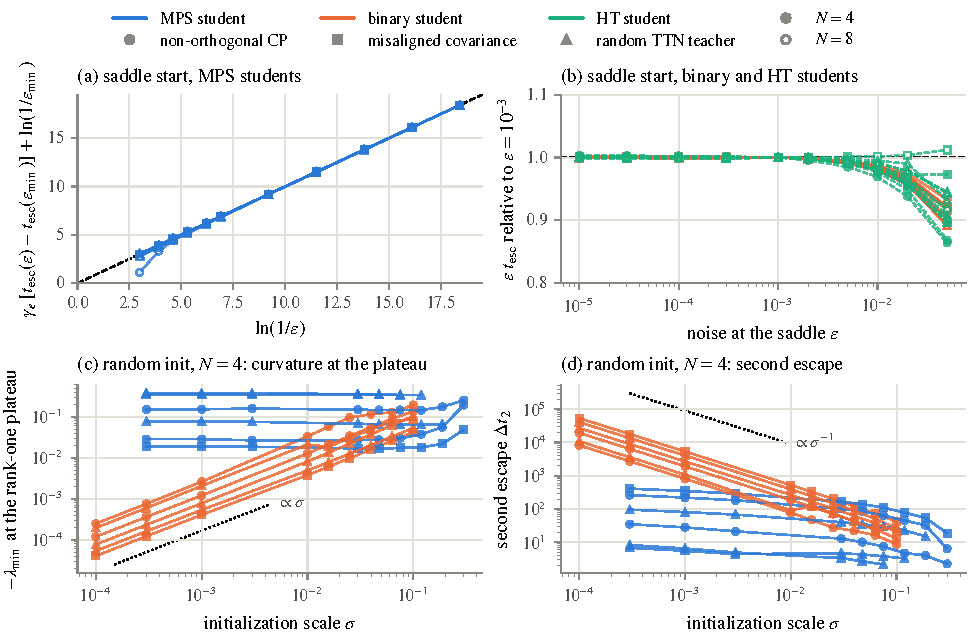
\includegraphics{data_teacher/contrast.pdf}
  \caption{One generic teacher, three trees. (a)~Saddle start, MPS students, 13 teachers: escape time
    rescaled by the predicted slope (mean over five seeds, $\gamma_e$ of the realized edge) against
    $\ln(1/\varepsilon)$; dashed: the prediction. (b)~Saddle start, binary and HT students, the same teachers
    except the misaligned one with $\Ns=8$, $\theta=20^\circ$: $\varepsilon\,t_{\rm esc}$ relative to its value at
    $\varepsilon=10^{-3}$ (per seed, then geometric mean); flat means $t_{\rm esc}\propto\varepsilon^{-1}$. (c),~(d)~Random
    initialization, the six teachers with $\Ns=4$ on MPS4 and binary4 (runs on the major rank-one saddle
    with a resolved plateau, geometric means over seeds): $-\lambda_{\min}$ of the gauge-projected Hessian at the
    plateau, and the second escape $\Delta t_2$. Takeaway: the same teachers give a strict saddle with a
    logarithmic escape at the predicted rate on the MPS, and a higher-order saddle
    ($\lambda_{\min}\propto\isc$, escape $\propto\varepsilon^{-1}$ or $\isc^{-1}$) on binary and HT trees.}
  \label{fig:dt-contrast}
\end{figure}

% ===========================================================================================
\subsection{Misaligned covariance}\label{sec:cov-misaligned}

The critical points, critical values and saddle types under a product covariance are those of the
whitened problem with teacher $\Sig^{1/2}\Wt$; escape rates are not, because the flow is preconditioned
\proven{} \newresult[for TTNs] (\cref{prop:A-precond}). With misaligned factors $\Sig^{1/2}\Wt$ is a
non-orthogonal CP teacher, with factors $\propto\Sigi i^{1/2}\fac ri$, while the escape is driven by $\Sig\Wt$, with
factors $\propto\Sigi i\fac ri$: the state must rotate after the escape, and misalignment alone can reverse the
order \derived{} \newresult{} (\cref{app:covariance}). Experiments \empirical{} ($d=\chi=4$, weights $(1,0.8)$,
$\beta\in\{0.5,1\}$, $\theta=0$--$45^\circ$, $\isc=0.05$ on binary4 and $0.1$ on MPS4, 20 seeds; an MPS4 sweep with $\beta=1$,
$\theta\in\{0,5,20\}^\circ$, nine $\isc$ from $3\cdot10^{-4}$ to $0.3$, ten seeds):
\begin{itemize}
  \item The first plateau is the predicted rank-one critical point of the $\Sig$-loss: median relative
    level errors $10^{-6}$--$10^{-3}$, median $\abs{\cos}\ge0.998$ with the critical tensor for $\theta\le30^\circ$, over
    the resolved plateaus (20--50\% of the MPS4 runs per $\theta$ have none at $\isc=0.1$).
  \item Early alignment with the race tensor (the best bond-rank-one approximation of $\Sig\Wt$), then
    realignment to the saddle \knownresult[in linear networks, binary4 being one:
    \citealp{atanasov2022neural}]: in $75$--$100\%$ of the binary4 runs at $\theta\ge10^\circ$, but on MPS4 only at
    $45^\circ$.
  \item Second escape on MPS4 (\cref{fig:dt-mps-laws}b) \newresult: $\isc^{-2.000}$ at $\theta=0$; at $20^\circ$ the log law
    (10 of 10 seeds) with slope $12.14\pm0.03$, below the bound $1/\abs{\lambda_{\min}}=12.31$ of its
    $\isc$-independent plateau curvature; at $5^\circ$ the log law (10 of 10) with $194.9\pm1.2$, approaching its
    bound $193.2$ from above (not yet asymptotic). The slope itself is not predicted: the head start under
    the preconditioned flow was not derived.
\end{itemize}

\begin{figure}[tbp]
  \centering
  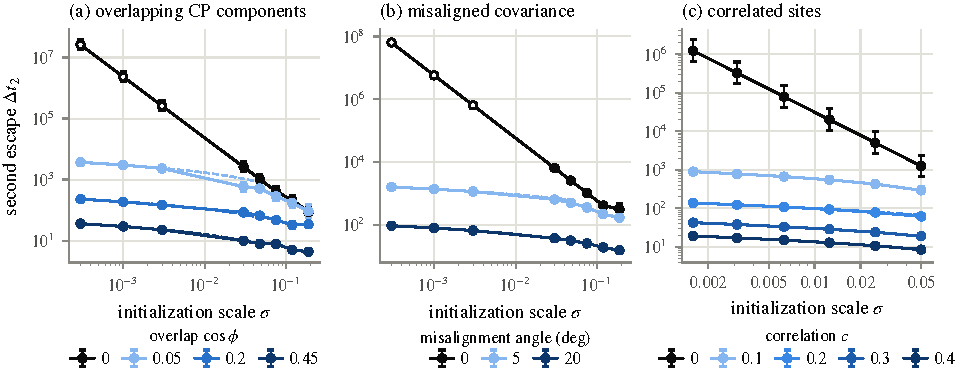
\includegraphics{data_teacher/mps_laws.pdf}
  \caption{MPS4 from random initialization: the second escape $\Delta t_2$ (onset events; runs on the major
    rank-one saddle with a resolved plateau; geometric mean over seeds with its standard error) when the
    teacher's components are made non-orthogonal in three ways. (a)~CP overlap $c$ ($d=4$, weights $(1,0.7)$,
    ten seeds); dashed: $h_e\ln(1/\isc)$ (\cref{cor:A-second-escape}), anchored at the smallest $\isc$ since the
    intercept is not predicted. (b)~Misaligned covariance at angle $\theta$ ($d=4$, ten seeds); dashed: slope
    $1/\abs{\lambda_{\min}}$, an upper bound. (c)~Correlated sites ($d=3$, four seeds); dashed: the two-stage law
    (\cref{app:covariance}; not computed for $\rho=0.1$, $0.3$). Black: the orthogonal baseline, dashed
    $\propto\isc^{-2}$; open markers: runs flagged by the float64-floor scan (dormant overlap $10^{-21}$--$10^{-12}$);
    without them the baseline exponents are $2.008\pm0.002$ ($c=0$) and $2.000\pm0.002$ ($\theta=0$). Takeaway: any
    non-orthogonality in the metric of the loss turns the $\isc^{-2}$ second plateau into a logarithmic
    one, with the predicted slope where there is a prediction.}
  \label{fig:dt-mps-laws}
\end{figure}

% ===========================================================================================
\subsection{Cross-site correlations}\label{sec:cov-correlated}

In the one-factor model $x^{(i)}=(1-\rho)^{1/2}z_i+\rho^{1/2}z_0$ (independent standard Gaussians; $\rho$ is the $c$
of \cref{app:covariance}) every site is whitened and two sites have covariance $\rho\Id$. The second-moment
matrix is not a product, so no whitening substitution exists; the loss is computed with the dense
matrix. The residual acquires \emph{pairing} tensors such as $(x^{(0)}\cdot x^{(1)})\,x^{(2)}_rx^{(3)}_r$, of bond
rank one on binary4 but $d$ on MPS4 \derived. On MPS4 the escape from the product saddle passes through
binary4's first plateau point, strict on MPS4 but of higher order on binary4, so the second plateau grows
by $\ln2\,[(1-\kappa_{\rm c})/\lambda_2+1/\lambda'']$ per halving of $\isc$: $2.128$ at $\rho=0.4$, $14.39$ at $\rho=0.2$ ($d=3$,
weights $(1,0.6)$) \derived{} \newresult{} (\cref{app:covariance}); binary4 stays at $\isc^{-1}$.
Experiments \empirical:
\begin{itemize}
  \item binary4 ($d=\chi=4$, weights $(1,0.7)$, $\isc=0.05$, 20 seeds): the first plateau falls from $0.33\,\Loss(0)$
    at $\rho=0$ to $0.29$, $0.20$, $0.14$, $0.10\,\Loss(0)$ at $\rho=0.2$--$0.5$, always at the predicted critical value
    (median relative error $\le5\cdot10^{-4}$): a blend with pairing terms, no longer a partial fit.
  \item Second escape \newresult{} (\cref{fig:dt-mps-laws}c; $d=3$, six $\isc$ from $0.0016$ to $0.05$, five seeds,
    events on the singular values across $01|23$): on MPS4 the log law in 4 of 4 seeds at every $\rho>0$ (seed 2 sits on
    the minor saddle and is excluded); increments per halving over the three smallest $\isc$ $2.133\pm0.003$
    at $\rho=0.4$ (predicted $2.128$) and $14.67\pm0.06$ at $\rho=0.2$ ($14.39$; $+2\%$, still falling), and
    $113.9\pm0.7$, $4.616\pm0.010$ at $\rho=0.1$, $0.3$ (no prediction computed); $\isc^{-2.000}$ at $\rho=0$. Binary4:
    $\isc^{-p}$, $p=1.005$--$1.011$. This repeats the theory's own check with more seeds: a replication, not
    an independent test.
  \item The MPS4 plateaus separate only logarithmically: separation ratio $2.6\to11$ at $\rho=0.4$ from
    $\isc=0.05$ to $0.0016$, against $14$--$19\to139$--$185$ on binary4.
  \item Online SGD (binary4, $\rho=0.3$, $\batch\ge256$, three seeds) crosses the same loss levels within $4\%$ of
    gradient flow.
\end{itemize}
HT students and $\Ns>4$ were not run with correlated inputs.

% ===========================================================================================
\subsection{Non-orthogonal CP teachers}\label{sec:teacher-cp}

The rank-one critical points are those of $g(x)=\ip{\bigotimes_ix_i}{\Wt}$ on unit rank-one tensors
\proven. With two components of equal weight and overlap $c$ at every site, an MPS has two rank-one
maxima (one near each component) iff $c<(\Ns-2)/\Ns$ and one blended maximum above \proven{} (among symmetric
points); unequal weights move the merger to a fold \derived; on binary4 the rank-one point is the top
singular pair of the $(01|23)$ matricization, a blend for every $c>0$ \newresult[elementary]
(\cref{prop:A-two-components}). The plateau is never a component. Experiments \empirical{} ($d=\chi=4$, weights
$(1,\tw2)$, $\tw2\in\{0.7,1\}$,
$c=0$--$0.8$, $\isc=0.05$ on binary4 and $0.1$ on MPS4, 20 seeds; an MPS4 sweep with $\tw2=0.7$,
$c\in\{0,0.05,0.2,0.45\}$, nine $\isc$ from $3\cdot10^{-4}$ to $0.3$, ten seeds):
\begin{itemize}
  \item MPS4 has two rank-one minima for $c\le0.45$ and one for $c\ge0.55$ ($\tw2=1$), two for $c\le0.35$ and
    one for $c\ge0.45$ ($\tw2=0.7$); binary4 one. First plateaus sit at these blends (median relative level
    errors $5\cdot10^{-5}$--$2\cdot10^{-3}$ on binary4, up to $3\%$ on barely resolved MPS4 plateaus; some binary4 runs
    with $\tw2=1$ sit at the second singular pair, a strict saddle), with levels falling as $c$ grows.
  \item Second escape on MPS4 (\cref{fig:dt-mps-laws}a) \newresult: $\isc^{-2.00}$ at $c=0$; for $c>0$ the log law (9 of
    9, 8 of 8, 8 of 8 seeds at $c=0.45$, $0.2$, $0.05$) with slopes $5.686\pm0.016$ ($h_e=5.682$), $34.40\pm0.20$
    ($34.14$) and $595\pm11$ ($570$; not yet asymptotic, as expected near the crossover overlap $c_\times=O(\isc)$
    of \cref{app:teachers}, a \conjecture), and an $\isc$-independent plateau curvature.
\end{itemize}
On binary4 the escape $\propto\isc^{-1}$ was measured for $c=0.2$ and $0.45$ only (\cref{sec:teacher-generic}).

% ===========================================================================================
\subsection{Random TTN teachers: plateaus are rank-constrained critical points}\label{sec:teacher-ttn}

With bond ranks fixed, the critical points are the fixed points of one-site alternating least squares
\proven{} \knownresult[in substance: \citealp{elden2011perturbation,holtz2012alternating}]
(\cref{prop:A-critical-points}); the hierarchical SVD is generically not one \proven{}
(\cref{prop:A-hsvd}). The
rank-one plateau should approach a local best rank-one approximation as $\isc^\alpha$, $\alpha=\min(\alpha_r,\alpha_a)$
(\conjecture: a heuristic crossing argument), and an MPS then gains rank bond by bond, first on
$e^*=\arg\max_e\sigma_2(M_e)$ with slope $h_{e^*}$ \derived. Experiments \empirical{} \newresult{} (MPS4 student,
$d=3$, $\chi=4$; five random MPS4 teachers with bond ranks $(2,3,2)$ and $\normF{\Wt}=1$; eight $\isc$ from
$10^{-3}$ to $0.2$; six seeds):
\begin{itemize}
  \item The rank-one plateau converges to the bond-rank-one critical point: per seed its distance
    falls as $\isc^\alpha$, $\alpha=0.72$, $0.83$, $0.41$, $0.93$, $0.80$ ($\pm0.01$--$0.03$), $0.07$--$0.15$ above the heuristic
    ($0.64$, $0.68$, $0.34$, $0.80$, $0.72$) for every teacher. For three teachers it is separated from every
    SVD-type truncation (hierarchical SVD, TT-SVD in both directions): at $\isc=10^{-3}$ it lies
    $10^{-4}$--$2.5\cdot10^{-3}$ from the critical point and $1.5\cdot10^{-3}$--$0.028$ from the nearest truncation
    (relative to $\normF{\Wt}$). For the other two teachers, and at the higher-rank plateaus, the critical
    point lies within $0.0032$ of an SVD-type truncation and the plateaus do not discriminate between them.
    (In CP factorization, small initialization follows a rank-one trajectory, \citealp{razin2021implicit}.)
  \item Ranks grow one bond at a time, e.g.\ $(1,1,1)\to(2,1,1)\to(2,2,1)\to(2,3,1)\to(2,3,2)$. The first increase
    after the rank-one plateau follows the log law in 26 of 26 seeds, with single-route slopes within
    $0.3$--$1.6\%$ of $h_{e^*}$ (e.g.\ $5.188\pm0.008$ against $5.175$), always on $e^*$ at $\isc=10^{-3}$; later increases
    were not timed. Gradient descent on tensor-train completion shows a plateau followed by abrupt
    rank growth \citep{milanesi2021implicit}.
\end{itemize}

% ===========================================================================================
\subsection{Teacher and student on different trees}\label{sec:teacher-mismatch}

A student bond must reach the rank of the teacher's matricization across it, bounded by products of
bond dimensions over cuts of the teacher's tree \proven{} \knownresult[standard min-cut bound; cf.\
\citealp{grasedyck2011introduction}, Lemmas~7--8] (\cref{app:teachers}):
a binary8 student of an MPS8 teacher of bond rank $r$ needs rank $\min(d^2,r^2)$ on the bonds of sites
$\{2,3\}$ and $\{4,5\}$. The routes give \emph{bottom-up order} \derived{} \newresult: the root bipartition
$\{0123\}|\{4567\}$ (the teacher's middle bond) has a three-core route only after both halves have bond
rank above one below it, so it grows only after a bottom bond on each half, whatever its teacher
Schmidt value. Experiments \empirical{} \newresult{} (binary8 student, $\chi=4$, twelve random MPS8 teachers
with bond ranks 2, $\isc=0.3$, $0.4$, $0.5$, eight seeds): in the 7 teachers whose root cut has a larger
teacher Schmidt value than both bottom bonds of a half, so that a weight order disagrees, bottom-up
order holds in 163 of 168 runs (56 of 56 at $\isc=0.3$), including 117 of 120 for five teachers whose root
cut is the strongest of all by $5.5$--$13\%$; the 5 exceptions grow the root after a bottom bond on one half
only. Over all 12 teachers: 249 of 256. ``Largest teacher Schmidt value first'' fails, and ``a sibling
pair first'' is no rule (8--100\% of the runs by teacher). Scope: $\Ns=8$, $\isc=0.3$--$0.5$. (An MPS8 student of
binary8 teachers at $\isc=0.45$ grows the predicted bond first in 2 of 24 runs; with $\ln(1/\isc)=0.8$ this is no
test of the asymptotic race of \cref{prop:A-agf-race}.)

% Summary table of Sec. 6.10, placed here so that it floats into the section.
\begin{table}[t]
  \centering
  \caption{Input covariance and teacher structure: what changes, and what predicts it. ``Escape'': the
    escape from the rank-one saddle.}
  \label{tab:cov-summary}
  \footnotesize
  \begin{tabularx}{\textwidth}{@{}>{\raggedright\arraybackslash}p{2.7cm}>{\raggedright\arraybackslash}X
      >{\raggedright\arraybackslash}p{4.0cm}@{}}
    \toprule
    complication & what changed (\empirical) & predicted by \\
    \midrule
    aligned covariance & quantitative only: order and times follow $\Lambda_r\tw r$, plateaus and swaps
      $\Lambda_r\tw r^2$; exponents unchanged & whitened problems with $\Lambda\tw{}$ (race) and $\Lambda^{1/2}\tw{}$
      (landscape) \\
    generic teachers & escape strict and logarithmic on MPS ($\le0.4\%$ from the saddle, $\le1.3\%$ from random
      init); $\propto\varepsilon^{-1}$, $\isc^{-1}$ on binary and HT & two-core routes and their rates \\
    misaligned covariance & plateaus at critical points of the $\Sig$-loss; early alignment (binary4); MPS4
      escape logarithmic & $\Sig^{1/2}\Wt$; slope only bounded \\
    cross-site correlations & binary4: first saddle with pairing terms; MPS4: logarithmic two-stage
      escape & two-stage law (replication) \\
    overlapping CP components & blended plateaus; MPS4 rank-one maxima merge at $c=1/2$; logarithmic
      escape & rank-one landscape; $h_e$ within $1\%$ ($c\ge0.2$) \\
    random TTN teachers & plateaus at rank-constrained critical points (3 of 5 teachers separated from
      SVD truncations); ranks grow bond by bond & critical points; $h_{e^*}$ within $1.6\%$ \\
    teacher on another tree & bottom-up order on binary8 (163 of 168 discriminating runs) & routes \\
    star teachers & larger learned component left iff $\lambda_{\max}(\Gamma)>\tw q$; log time on MPS4, polynomial
      on HT4 & piggyback graph; rates within $0.2\%$ \\
    real data & pending (\cref{sec:real-data}) & -- \\
    \bottomrule
  \end{tabularx}
\end{table}

% ===========================================================================================
\subsection{Star teachers: forgetting a learned component}\label{sec:teacher-star}

A learned component $j$ without a two-core route to the rest is a strict saddle iff
$\lambda_{\max}(\Gamma)>\tw j$, $\Gamma$ the weighted adjacency matrix of the piggyback graph, and then
$\lambda_{\min}=-q_j^{\Kc-2}(\lambda_{\max}(\Gamma)-\tw j)$ \proven{} \newresult[for general trees; deep linear networks:
\citealp{achour2024loss}, Thm~7] (\cref{prop:A-piggyback-graph}). The \emph{star} has $q=0000$ ($\tw q=2$) and
$r=1010$, $r'=1001$ (weight $w$ each, $d=2$), which share the piggyback node: $\lambda_{\max}(\Gamma)=\sqrt2\,w$, so
``$q$ learned'' ($\params_q$) is strict iff $w>\sqrt2$, although both residual components are smaller and each
needs three or more cores. Experiments ($\chi=3$; MPS4, binary4, HT4; saddle start at $\params_q$ with
$\varepsilon=10^{-6}$--$10^{-2}$, five seeds; random initialization at $w=1.2$, $1.6$, ten seeds):
\begin{itemize}
  \item \emph{Hessian} \proven{} and computed: the formula holds to $10^{-15}$ on MPS4, binary4, HT4 and a
    binary8 analogue ($-0.3716$, $-0.3310$, $-0.4311$, $-0.4311$ at $w=1.6$); no negative eigenvalue for $w\le1.40$.
    This repeats the theory's check; binary4 is a deep linear network, where it is known.
  \item \emph{Threshold} \empirical{} \newresult[dynamics]: at $\varepsilon=10^{-6}$ no seed leaves $\params_q$ at
    $w=1.4138$ ($\lambda_{\max}(\Gamma)/\tw q=0.9998$) and all do at $1.4146$ ($1.0003$), on MPS4 and binary4; on HT4
    the step lies between $1.40$ and $1.42$ for $\varepsilon\le10^{-3}$. At $\varepsilon=10^{-2}$ it moves to $1.43$--$1.44$: near the
    threshold the strict escape is slow and the polynomial route that adds $r$ wins at moderate noise.
  \item \emph{One or two strict stages} \derived{} (from the computed Hessians) and \empirical{}
    \newresult: the slope of the escape time against $\ln(1/\varepsilon)$ is $1/\abs{\lambda_q}$ within $0.21\%$ where the
    event times one strict stage ($w\ge1.48$ on all trees, every $w$ on binary4). Near the threshold on MPS4
    the flow stops at a blended rank-one point that keeps $\ov q=0.98$, $0.93$ ($w=1.42$, $1.44$) and is itself
    strict: the measured $130.0\pm0.2$ and $29.39\pm0.02$ equal $1/\abs{\lambda_q}+1/\abs{\lambda_b}=129.9$ and $29.3$ (one stage:
    $86.4$, $19.4$). On HT4 that point has no negative eigenvalue, and leaving it takes a time $\propto\varepsilon^{-1}$
    ($p=0.995$, $0.998$; at $w=1.6$, $\ov q<\frac12$ after $3.4\cdot10^3$, $3.3\cdot10^4$, $3.3\cdot10^6$ for $\varepsilon=10^{-3}$, $10^{-4}$,
    $10^{-6}$). A star forgets $q$ in logarithmic time on MPS4 and binary4 but polynomially on HT4: the tree
    contrast of \cref{sec:teacher-generic} again.
  \item \emph{Random initialization} \empirical{} \newresult{} ($w=1.6$; $\isc=0.01$--$0.1$ on MPS4, $0.005$--$0.05$ on
    binary4):
    the flow never sits at $\params_q$ (at most $0.13$ time units at its loss level, one seed $1.7$; up to 538
    at ``$q$ forgotten''). The initialization direction sets the class: $q$ learned last (binary4 7 of 10
    seeds, MPS4 1 of 10), $\ov q$ rising to $0.78$--$1.00$ and decaying (3, 4 of 10), or a blended start with
    $\ov q\le0.68$ (MPS4, 5 of 10). The decay deepens steeply as $\isc$ decreases, not as a power law; $q$ is
    relearned last. Sub-critical stars ($w=1.2$) keep $q$ ($\min\ov q\ge0.992$).
\end{itemize}
\emph{Withdrawn:} the laws $\min\ov q\propto\isc^{5.7\pm0.3}$ and a relearning time $\propto\isc^{-1.4}$ from random
initialization; they pooled two classes of runs, dropped the points where $\ov q$ crosses zero, and
describe runs that never visit $\params_q$.

% ===========================================================================================
\subsection{Real data}\label{sec:real-data}
\placeholder{To be written when the real-data experiment (PLAN.md B5: MNIST with quadtree, MPS and
scrambled-site trees) is finished.}
% TODO(real-data): another agent writes this subsection. Question: which of the effects above survive
% real inputs (non-Gaussian, correlated pixels, unknown teacher): the plateau structure and its scaling
% with sigma, the order of bond-rank growth, and the dependence on the tree (quadtree vs MPS vs
% scrambled sites). Settings go to Appendix B and figures to Appendix C, as for the other experiments.

% ===========================================================================================
\subsection{Summary}\label{sec:cov-summary}

Only the aligned covariance leaves the qualitative picture unchanged (\cref{tab:cov-summary}). Every
other complication breaks the orthogonality of the teacher's components in the metric of the loss, and
then the student's tree decides whether the escape from the rank-one saddle is logarithmic (MPS) or
polynomial (binary, HT). The baseline theory predicts each change after the substitution in the
table, except the slope under a misaligned covariance from random initialization, which is only
bounded.
